\documentclass{beamer}
\pdfstringdefDisableCommands{%
  \def\\{}%
  \def\texttt#1{<#1>}%
}
\beamertemplatenavigationsymbolsempty


% Footnote
\setbeamertemplate{footline}{\leavevmode%
  \begin{beamercolorbox}[wd=.33\paperwidth,left,ht=2.5ex,dp=1.5ex,rightskip=4pt plus 1pt, leftskip=4pt]{subsection in head/foot}
    Team 12
  \end{beamercolorbox}%
  \begin{beamercolorbox}[wd=.33\paperwidth,center,ht=2.5ex,dp=1.5ex]{section in head/foot}
  \end{beamercolorbox}%
  \begin{beamercolorbox}[wd=.34\paperwidth,ht=2.5ex,dp=1.5ex,leftskip=4pt plus 1pt,rightskip=4pt plus 1pt]{subsection in head/foot}
    \hfill\insertframenumber/\inserttotalframenumber
  \end{beamercolorbox}%
}


\title{Stato di avanzamento}
\subtitle{Sprint 3}
\author{
  \texorpdfstring{\parbox{45mm}{\centering\scriptsize Zaid Cheikh Ibrahim \\[-0.3em] {\tiny PO Operativo}}}{} \and 
  \texorpdfstring{\parbox{45mm}{\centering\scriptsize Tian Cheng Xia \\[-0.3em] {\tiny Scrum master}}}{}\\[1em]
  \texorpdfstring{\parbox{45mm}{\centering\scriptsize Qun Hao Henry Lee \\[-0.3em] {\tiny Developer}}}{} \and 
  \texorpdfstring{\parbox{45mm}{\centering\scriptsize Manuel Paris \\[-0.3em] {\tiny Developer}}}{}\\
}
\institute{
  Corso di Ingegneria del Software\\
  Alma Mater Studiorum $\cdot$ Università di Bologna  
}
\date{5 dicembre 2022}


\begin{document}

{
\setbeamertemplate{footline}{} 
\begin{frame}
  \titlepage
\end{frame}
}
\addtocounter{framenumber}{-1}

\begin{frame}
  \frametitle{Obiettivi dello sprint}
  \begin{itemize}
    \item Implementare le pagine per L'Eredità e Reazione a Catena
    \item Iniziare l'implementazione degli scacchi
  \end{itemize}
\end{frame}

\begin{frame}
  \frametitle{Use case (1/2)}
  \begin{figure}
    \centering
    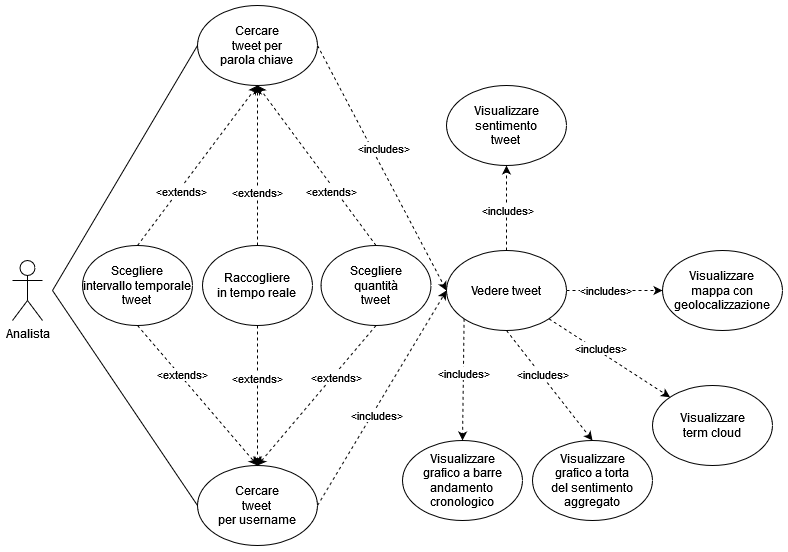
\includegraphics[width=\textwidth]{./img/usecase.tweet.png}
  \end{figure}
\end{frame}

\begin{frame}
  \frametitle{Use case (2/2)}
  \begin{figure}
    \centering
    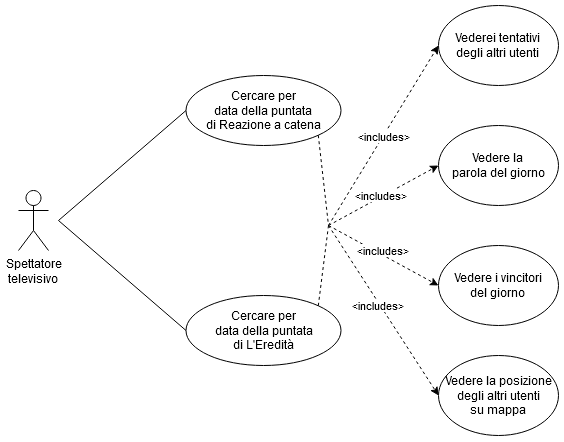
\includegraphics[height=170px]{./img/usecase.tvgame.png}
  \end{figure}

  \begin{figure}
    \centering
    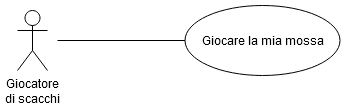
\includegraphics[height=40px]{./img/usecase.chess.png}
  \end{figure}
\end{frame}

\begin{frame}
  \frametitle{Retrospettiva}
  \begin{figure}
    \centering
    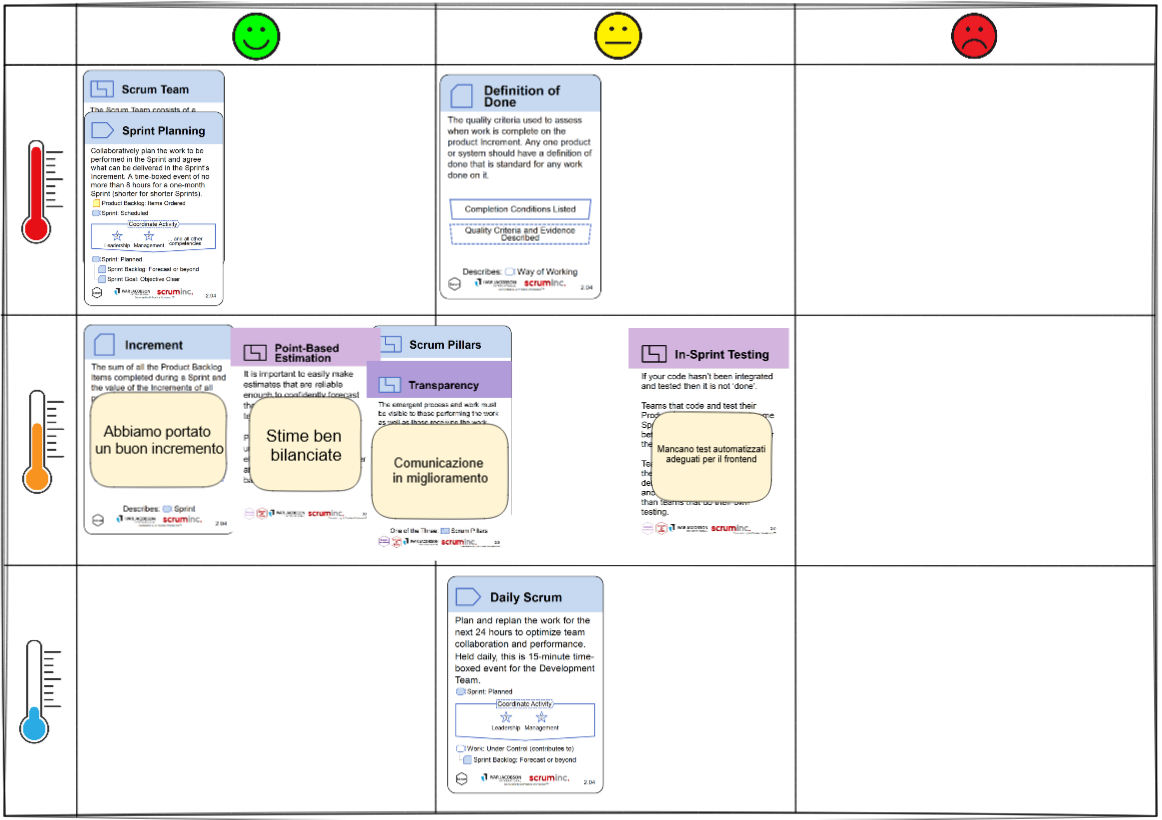
\includegraphics[width=\textwidth]{./img/retrospettiva.png}
  \end{figure}
\end{frame}

\begin{frame}
  \frametitle{Testing}
  \begin{figure}
    \centering
    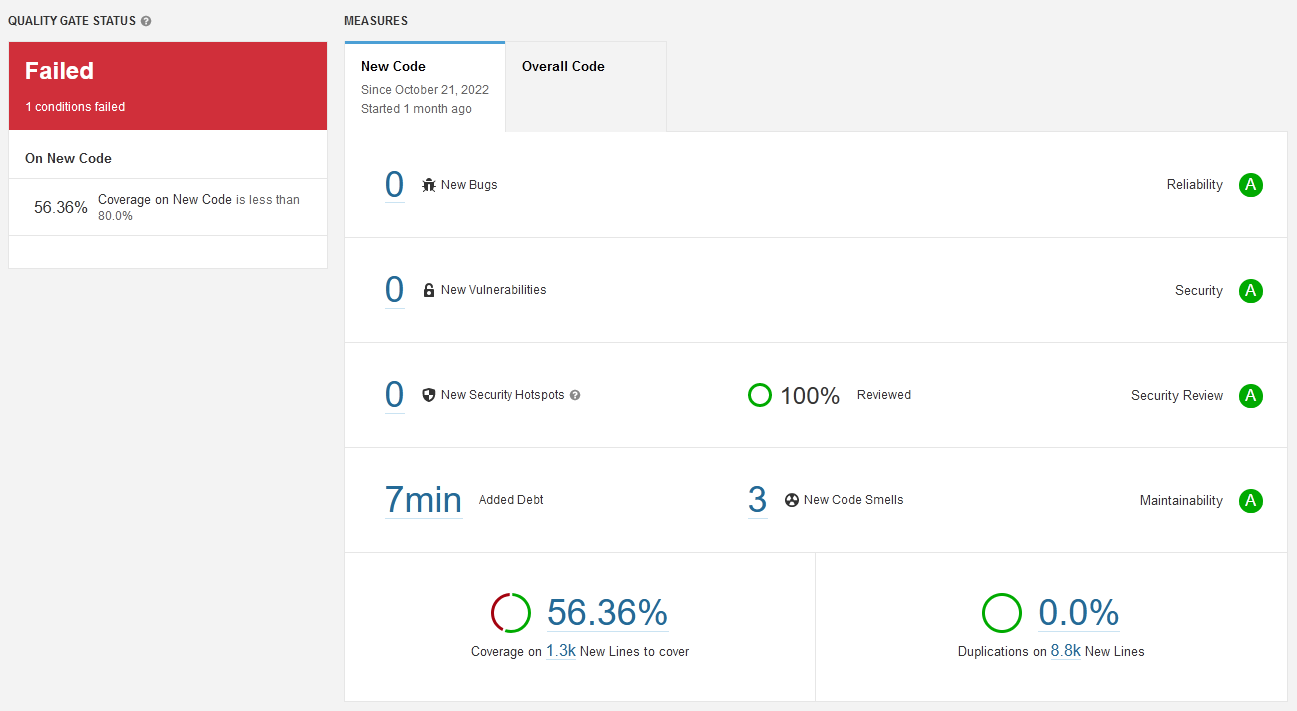
\includegraphics[width=\textwidth]{./img/sonarqube.png}
  \end{figure}
\end{frame}

\begin{frame}
  \frametitle{Stato attuale}
  \begin{itemize}
    \item Pagine per L'Eredità e Reazione a Catena
    \begin{itemize}
      \item  Selezionare la data di trasmissione
      \item  Visualizzare i tentativi degli altri utenti
      \item  Visualizzare la parola del giorno
      \item  Visualizzare gli utenti che indovinano la parola
      \item  Visualizzare la posizione degli utenti
    \end{itemize}
    \item Pagina per lo scacchi con la possibilità di giocare la propria mossa
  \end{itemize}
  \begin{figure}
    \centering
    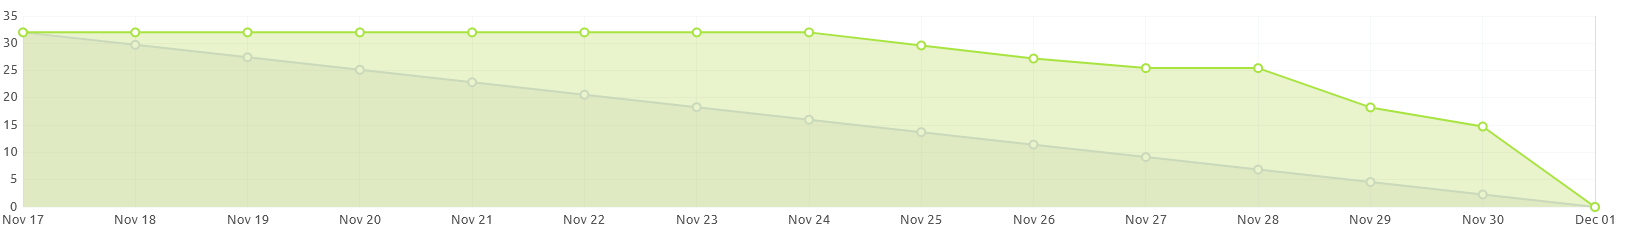
\includegraphics[width=\textwidth]{./img/burndown.png}
    \caption{Burndown sprint 3}
  \end{figure}
\end{frame}

\end{document}